\chapter{Sensor data and usage} \label{chap:sensordataandusage}%overvej ny titel, måske bare Sensors
This chapter's goal is to explain, in more detail, how the sensor data is utilized most appropriately. 

\section{Compass calibration}
The compass in an IMU is very unstable, though reasonably reliable when at rest, due to the soft and hard iron core distortion caused by varying and permanent magnetic fields surrounding the sensor \cite{magnetometercorrections}. For example, from nearby components on the PCB or the propeller motor.
Therefore, to maximize the stability and precision of the estimations of roll, pitch, and yaw of the drone, the IMU must be calibrated accordingly.
The IMU's magnetometers will be calibrated with the method of Kris Winer\cite{compasscalib}. A well-calibrated compass will output data in a sphere, as small as possible, centered around $[x,y,z]=[0,0,0]$.\\
The calibration routine consists of waving each PCB such that it faces and moves in every direction. Magnetometer measurements are made during the routine to determine its minimum and maximum output values. These values will decide the soft iron core scaling bias.\\
Furthermore, measurements for x, y and z are averaged with the duration of the routine to generate the hard iron core offset biases.\\
Additionally, the factory axis sensitivity adjustment values are read from the compass ROM. \\
An example of realistic measurements from an uncalibrated compass can be seen in fig. \ref{fig:uncalibcompass}. Followingly, example measurements from a calibrated magnetometer are in fig. \ref{fig:calibcompass}.

\begin{figure}[h!]
    \centering
    \begin{minipage}[t]{0.48\textwidth}
        \centering
        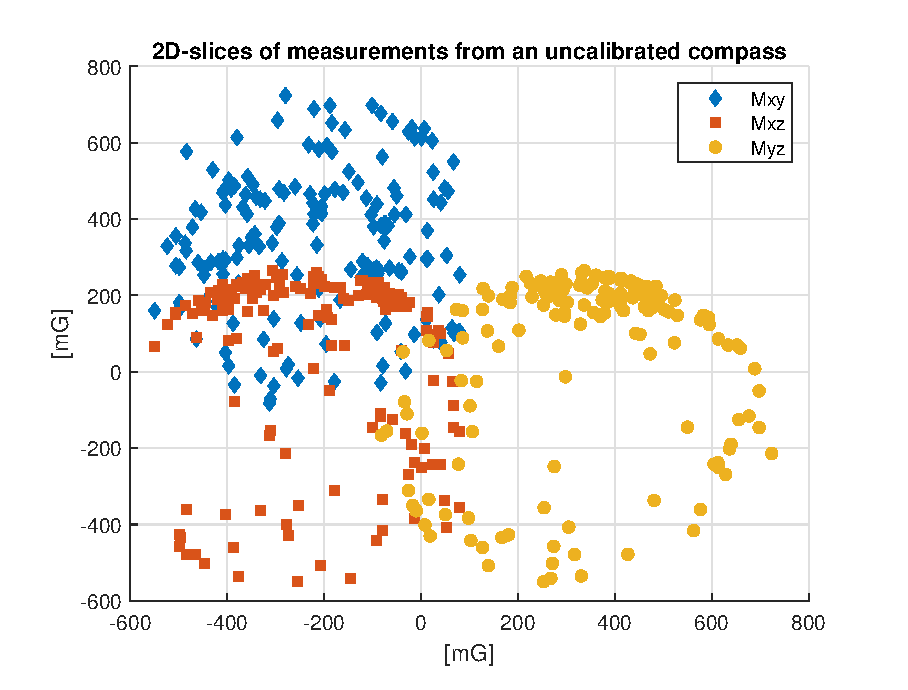
\includegraphics[width=0.96\textwidth]{figures/sensors/board3_uncalibrated_scatterplot.eps}
        \caption{Uncalibrated 2D-slice measurements from the magnetometer on \texttt{arm 3}}
        \label{fig:uncalibcompass}
    \end{minipage}%
    \hspace{.03\textwidth}
    \begin{minipage}[t]{0.48\textwidth}
        \centering
        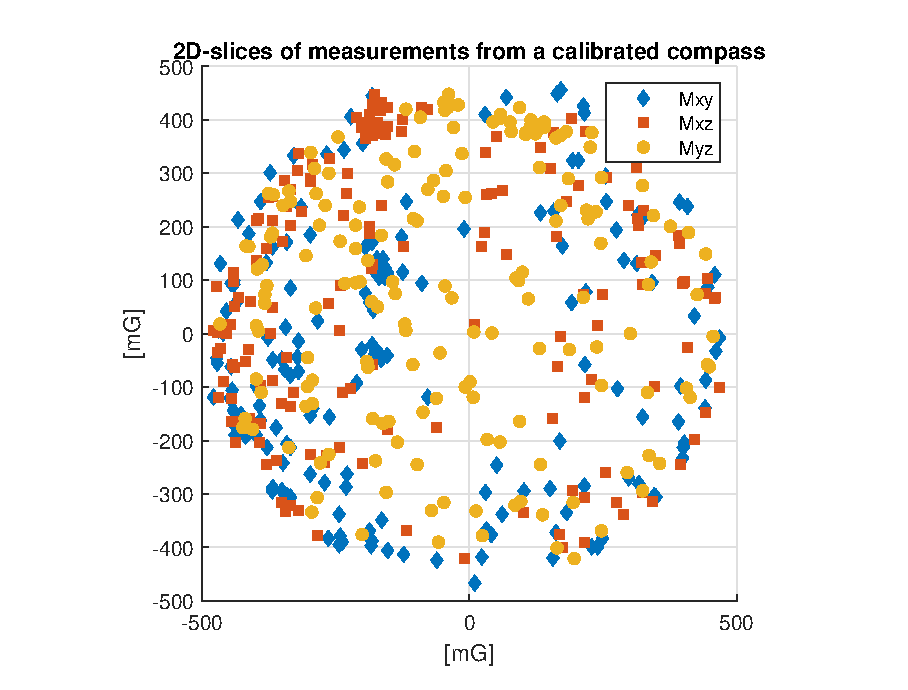
\includegraphics[width=0.96\textwidth]{figures/sensors/board3_calibrated_scatterplot.eps}
        \caption{Calibrated 2D-slice measurements from the magnetometer on \texttt{arm 3}}
        \label{fig:calibcompass}
    \end{minipage}
\end{figure} 

\section{Drone orientation}
The orientation of the drone is found by using measurements from the IMU and a sensor fusion algorithm. When working with orientation in 3 dimensions, Euler angles are typically used, but for this application with a continuous rotation object, quaternions are preferred. Euler angles are three angles used to describe the orientation of a rigid body with regards to a fixed coordinate system. The sequence and axis of which the rotations are made, changes the angles, and thus a convention must exist. In aerospace, the most common one is 'Tait-Bryan' angles. It is from this convention that the names roll, pitch and yaw originate. Euler angles are an easy and intuitive way to describe orientation, but have its disadvantages. Further details of Euler angles will not be discussed, only how they fare compared to quaternions. The difference between quaternions and Euler angles will be analyzed, after a brief introduction of quaternions.\\ 


Quaternions are 4-dimensional vectors, with four real coefficients and three imaginary components, typically denoted with i, j, k, usually on the following form:
\begin{equation*}
    \textbf{q} = [q_0, q_1, q_2, q_3] = a + bi + cj + dk
\end{equation*}
where a, b, c, d are real numbers. It can be seen as a scalar \textit{a}, and a three dimensional vector $bi + cj + dk$ . Like regular complex numbers, they can be written on different forms. Quaternions can be used for many things, but are especially useful for describing orientation of 3D objects. When using quaternions for describing rotations, they must be of unit length. When of unit length, the quaternions describe a 3D space on the surface of a hypersphere. Each point on the hypersphere described by a unit quaternion corresponds to a rotation of a 3D object. 
Additional details about quaternions and how they work will not be discussed further, only how they relate to Euler angles.\\

Quaternions are superior to Euler angles for describing rotating objects, especially ones that laps themselves. This is both due to dealing with edge cases like going from 0 to 360 degrees when completing a full rotation, but they also resolve the problem of singularities. Singularities occur with Euler angles when two angles align. This might happen when the second angle moves in such a way that the first and third angle align, losing one degree of freedom. A third benefit is their improved accuracy when integrating over incremental changes in attitude over time \cite{JamesDiebelQuaternions}. \\
%In the control loops for wing tilt, a quaternion based approach will be used, to maintain the benefits compared to traditional Euler angles.\\
As mentioned, when using quaternions to describe rotations, it is essential to note that they are of unit length. The length of a quaternion is found as in equation \ref{eq:normquaternion}. 

\begin{equation} \label{eq:normquaternion}
    ||q|| = \sqrt{q_0^2 + q_1^2 + q_2^2 + q_3^2}
\end{equation}

When converting from unit quaternions to Euler angles, it is crucial to note the sequence of angles. The microcontroller runs a library written by Kris Winer, that utilizes quaternions, such that a stable orientation can be read from the IMU \cite{kriswinermpu9250}. The library implements two filter fusion algorithms: Madgwick and Mahony filters. For converting between quaternions and Euler angles, the library uses 'Tait-Bryan' notation, which also is known as a 1,2,3 sequence \cite{JamesDiebelQuaternions}.
With this notation, the series of calculations is yaw, then pitch, then roll. If the order of rotation is changed, the result is an entirely different set of angles. 

Eq. \ref{eq:uq2ea1}, \ref{eq:uq2ea2} and \ref{eq:uq2ea3} are the equations used by Kris Winer for converting unit quaternions to Euler angles. 
\begin{align} \label{eq:uq2ea1}
      yaw = \psi &= arctan\left(2\cdot (q_1 q_2 + q_0 q_3), \, q_0^2 + q_1^2 - q_2^2 - q_3^2    \right)\\\label{eq:uq2ea2}
    pitch = \theta &= -arcsin\left(  2\cdot(q_1 q_3 -q_0 q_2)   \right)\\
     roll = \phi &= arctan\left( 2\cdot (q_1 q_2 +q_2 q_3), \, q_0^2 -q_1^2 -q_2^2 +q_3^2 \right)\label{eq:uq2ea3}
\end{align}
As noted in the library, for the IMU's coordinate system, positive z-direction is down towards earth, resulting in a positive sign of the gravitational force. With the local declination of the earth's magnetic field taken into account, yaw is the angle between the sensor's x-axis and the true North. 
Pitch is the angle between the sensor's x-axis and the earth's ground plane, towards the earth is positive. Roll is the angle between the sensor's y-axis and the earth's ground plane, towards the earth is negative \cite{kriswinermpu9250}.

As for the filter fusion algorithm, the microcontroller runs Kris Winer's implementation of a Madgwick filter. This filter combines all data from the IMU (accelerometer, gyroscope, and magnetometer) and calculates the unit quaternions that describe the IMU's absolute orientation. 
A Mahony filter was considered, as well. Kris Winer describes the Mahony filter, as similar to the Madgwick filter, but with proportional and integral filtering on the error \cite{quaternionFilters}. This could potentially result in a filter with less drift of values compared to the Madgwick filter. The drone experienced the best performance with the Madgwick filter. This is also supported by at least one source that compared the two \cite{madgwickvsmahony}. The sensitivity of the gyroscope is set to 2000 DPS, which corresponds to approximately six full rotations per second. 
% link: https://x-io.co.uk/open-source-imu-and-ahrs-algorithms/

\section{Chapter summary}
The IMU was calibrated to fit its measurements more accurately to the drone's position. Euler angles and quaternions were introduced, and their pros and cons discussed. Two filter fusion algorithms were presented, as a way of estimating the drone's orientation. The objectives outlined in section \ref{sensorgoals} have been analyzed and are ready to be tested. The performance will be assessed in section \ref{results:measurementprecision}. 